% pdflatex
% chktex-file 1
% chktex-file 11
% chktex-file 12
% chktex-file 13
% chktex-file 36

\documentclass[10pt,hyperref={colorlinks,citecolor=blue,urlcolor=peking_blue,linkcolor=}]{beamer}

\setbeamerfont{frametitle}{size=\large}
\setbeamerfont{block title}{size=\normalsize}
\setbeamerfont{block body}{size=\small}
\setbeamerfont{itemize/enumerate body}{size=\small}
\setbeamerfont{itemize/enumerate subbody}{size=\footnotesize}

\usepackage{PekingU}
\usefonttheme{serif}
%\usepackage[scheme = plain]{ctex}
\usepackage{hyperref}
\usepackage{charter} % Nicer fonts
% other packages
\usepackage{latexsym,amsmath,xcolor,calligra}
\usepackage{amsfonts} 
\usepackage{bm}

\usepackage{siunitx}
\sisetup{per-mode=symbol}

\usepackage{graphicx}
\usepackage{caption} 
\usepackage{wrapfig}

\usepackage{natbib}

\usepackage{ragged2e}
\usepackage{parskip}

\usepackage{booktabs}
\usepackage{makecell}
\usepackage{multirow}
\usepackage{multicol}

\apptocmd{\frame}{}{\justifying}{} % Allow optional arguments after frame.

\newcommand{\theHalgorithm}{\arabic{algorithm}}
\theoremstyle{plain}
\newtheorem{axiom}{Axiom}
\newtheorem{claim}[axiom]{Claim}
\newtheorem{assumption}{Assumption}
\newtheorem{remark}{Remark}
\newtheorem{proposition}{Proposition}
\setbeamertemplate{theorems}[numbered] 


\author[Yizhan Feng]{Yizhan Feng}
\title{Genetic Diversity Analysis in Homologous Genes of Mammals and Humans}
\subtitle{Using \textit{ALDH2} and \textit{TAS2R38} Genes as Examples}
\institute{Yuanpei College, Peking University}
\date{2025/10/31}

\newif\ifplacelogo % create a new conditional
\placelogotrue % set it to true
\logo{
\ifplacelogo
\includegraphics[width=2cm]{../Figures/PKU-China-logo.png}
\fi
}
% official colors match with the PKU red
\def\cmd#1{\texttt{\color{red}\footnotesize $\backslash$#1}}
\def\env#1{\texttt{\color{blue}\footnotesize #1}}
\definecolor{deepblue}{rgb}{0,0,0.5}
\definecolor{deepred}{rgb}{0.6,0,0}
\definecolor{deepgreen}{rgb}{0,0.5,0}
\definecolor{halfgray}{gray}{0.55}

\begin{document}
{
\setbeamertemplate{logo}{}
\begin{frame}
    \titlepage
    \begin{figure}[htpb]
        \begin{center}
            
\includegraphics[width=0.2\linewidth]{Figures/PKUlogo.png}
        \end{center}
    \end{figure}
\end{frame}
}

\placelogofalse

\section{Introduction}

\begin{frame}{Genetic Diversity: The Foundation of Evolution}
    \begin{block}{The Significance of Genetic Variation}
        \begin{itemize}
            \item Genetic diversity is the raw material for \textbf{evolution and adaptation}
            \item Single nucleotide polymorphisms (SNPs) account for most genetic variations in populations
            \item Understanding genetic diversity helps elucidate:
            \begin{itemize}
                \item Evolutionary history and phylogenetic relationships
                \item Population migrations and demographic events
                \item Disease susceptibility and pharmacogenetics
            \end{itemize}
        \end{itemize}
    \end{block}

    \begin{block}{Model Genes for Diversity Studies}
        \begin{itemize}
            \item \textbf{\textit{ALDH2}}: Aldehyde dehydrogenase, crucial in alcohol metabolism
            \begin{itemize}
                \item rs671 (Glu504Lys) shows strong East Asian-specific distribution
                \item Associated with alcohol flush reaction and disease risks
            \end{itemize}
            \item \textbf{\textit{TAS2R38}}: Bitter taste receptor for PTC/PROP compounds
            \begin{itemize}
                \item Classic example of balanced polymorphism in human populations
                \item Three linked SNPs determine taste sensitivity phenotypes
            \end{itemize}
        \end{itemize}
    \end{block}
\end{frame}

\begin{frame}{Research Objectives and Approach}
    \begin{block}{Methodological Framework}
        \vspace{-0.7em}
        \hspace{0.4em}
        \begin{columns}
            \begin{column}{0.9\textwidth}
                \textbf{Experimental Approach:}
                \begin{itemize}
                    \item DNA extraction from buccal swabs
                    \item PCR amplification of target regions
                    \item Sanger sequencing for genotype determination
                \end{itemize}

                \textbf{Bioinformatic Analysis:}
                \begin{itemize}
                    \item Homologous sequence retrieval
                    \item Multiple sequence alignment
                    \item Phylogenetic tree construction
                \end{itemize}
            \end{column}
        \end{columns}
        \hspace{1em}
    \end{block}
\end{frame}

\section{Methods}

\begin{frame}{Phenotypes Survey and Genes Extraction}
    \begin{block}{Phenotype Assessment}
        \begin{itemize}
            \item \textbf{Taste sensitivity}: PTC/PROP test strips for bitter taste perception
            \item \textbf{Aldehyde metabolism}: Recorded based on personal experience
        \end{itemize}
    \end{block}

    \begin{block}{Genomic DNA Extraction}
        %\vspace{0.2em}
        %\setlength{\columnsep}{1em} % 增加列间距
        \begin{columns}
            \hspace{1em} % 添加左边距
            \begin{column}{0.38\textwidth} % 稍微减小列宽
                
                \textbf{Sample Collection:}
                \begin{itemize}
                    \item Buccal swabbing
                    \item Two samples per person
                    \item Air-dried in envelopes
                \end{itemize}
            \end{column}

            \hspace{-2em}
            
            \begin{column}{0.58\textwidth}
                
                \textbf{Extraction Protocol:}
                \begin{itemize}
                    \item Proteinase K digestion
                    \item DNeasy Mini Spin Column purification
                    \item Elution in Buffer AE (\qty{50}{\ul})
                \end{itemize}
            \end{column}
        \end{columns}
    \end{block}

    \begin{block}{Quality Control}
        \begin{itemize}
            \item \textbf{Spectrophotometry}: NanoDrop concentration measurement
            \item \textbf{Electrophoresis}: 1\% agarose gel, \qty{120}{\V}, 1 kbp ladder
            \item \textbf{Storage}: Diluted to \qty{5}{\ng \per \uL} in Buffer AE
        \end{itemize}
    \end{block}
\end{frame}

\begin{frame}{PCR Amplification}

    \begin{block}{Primer Design and Preparation}
        \begin{itemize}
            \item \textbf{Target genes}: \textit{ALDH2} and \textit{TAS2R38}
            \item \textbf{Mutation sites}: 
            \begin{itemize}
                  \item \textit{ALDH2}: Position 1,510
                  \item \textit{TAS2R38}: Positions 145, 785, 886
            \end{itemize}
            \item \textbf{Primer design}: Using Benchling Primer3 tool + universal M13 tails
            \item \textbf{Amplicon size}: $200\sim500$ bp
        \end{itemize}
    \end{block}
    
    \begin{block}{PCR Amplification}
        \vspace{0.3em}
        \begin{columns}
            \hspace{0.5em}
            \begin{column}{0.58\textwidth}
                \textbf{Reaction Setup:}
                \begin{itemize}
                    \item \qty{15}{\ul} volume each (Primer + Template + dNTP + Mg$^{2+}$ + TaqGold + Solvent)
                    \item 2 templates $\times$ 3 primers $\times$ 2 duplicates = 12 samples 
                    \item Blank control (water as template)
                \end{itemize}
            \end{column}
            \hspace{-2.5em}
            \begin{column}{0.36\textwidth}
                \textbf{Thermal Cycling:}
                \begin{itemize}
                    \item Touchdown protocol
                    \item $60\to\qty{50}{\celsius}$ annealing ($-\qty{2}{\celsius}$ every 2 cycles) \& 42 final cycles
                    \item $2.5\sim3$ hours total
                \end{itemize}
            \end{column}
        \end{columns}
    \end{block}
\end{frame}


\begin{frame}{Sequencing and Phylogenetic Study}

    \begin{block}{Analysis and Sequencing}
        \begin{itemize}
        \item \textbf{Electrophoresis}: 1.5\% agarose gel, \qty{120}{\V}, 100 bp Ladder
        \item \textbf{Sequencing}: 6 samples (clear bands \& correct length) sent for sequencing 
        \item \textbf{Analysis}: Retrieve sequence and identify genotypes of each sample
        \end{itemize}
    \end{block}

    \begin{block}{Phylogenetic Tree Construction}
        \begin{itemize} 
            \item \textbf{Homologous sequences}: Downloaded \textit{ALDH2} \& \textit{TAS2R38} CDS from UCSC/NCBI ($\geq10$ species)
            \item \textbf{Phylogeny}: Construct phylogenetic using MEGA 12
            \item \textbf{Constructing Methods}: Neighbor-joining (NJ), Maximum Parsimony (MP), Maximum Likelihood (ML) 
        \end{itemize}
    \end{block}
\end{frame}

\section{Results}

\begin{frame}{Survey on Phenotypes}
    \vspace{-1em}
    \begin{table}[H]
        \centering
        %\renewcommand{\arraystretch}{2} 
        %\setlength{\extrarowheight}{5pt}
        \scriptsize
        \begin{tabular}{>{\raggedright\arraybackslash}p{0.2cm}>{\raggedright\arraybackslash}p{0.7cm}>{\raggedright\arraybackslash}p{3.5cm}>{\raggedright\arraybackslash}p{2.6cm}>{\raggedright\arraybackslash}p{1.7cm}}
            \toprule
            \textbf{No} & \textbf{Name} & \textbf{Self-reported Alcohol Metabolism Ability} & \textbf{Bitter Taste Self-perception} & \textbf{Bitter Test Strip (1$\sim$5)} \\
            \midrule
            \makecell{1} & \makecell[l]{Le \\ Zhang} & \makecell[l]{Drinks occasionally, rarely flush; \\ from Shaanxi; \\ parents do not flush} & \makecell[l]{No distinct sensation \\ when eating cruciferous \\ vegetables} & \makecell[l]{Slightly bitter, \\ 1$\sim$2} \\[12pt]
            
            \makecell{2} & \makecell[l]{Jinlin \\ Liu} & \makecell[l]{Drinks occasionally, rarely flush; \\ from Hunan; \\ both parents flush easily} & \makecell[l]{Enjoys eating \\ cruciferous  vegetables} & \makecell[l]{Slightly bitter, \\ 1} \\[12pt]
            
            \makecell{3} & \makecell[l]{Xiangyu \\ Han} & \makecell[l]{No alcohol consumption; \\ from Shandong; \\ father flushes when drinking, \\ mother does not drink} & \makecell[l]{Enjoys eating \\ cruciferous vegetables} & \makecell[l]{Somewhat bitter, \\ 2} \\[15pt]
            
            \makecell{4} & \makecell[l]{Xinyu \\ Jiang} & \makecell[l]{No alcohol consumption; \\ from Jiangxi; \\ father flushes when drinking, \\ mother does not drink} & \makecell[l]{Enjoys eating \\ cruciferous vegetables} & \makecell[l]{Somewhat bitter, \\ 1} \\[15pt]
            
            \makecell{5} & \makecell[l]{Yizhan \\ Feng} & \makecell[l]{Moderate flushing when drinking; \\ from Zhejiang; \\ cannot recall if parents flush} & \makecell[l]{Enjoys eating \\ cruciferous vegetables} & \makecell[l]{Somewhat bitter, \\ 1} \\
            \bottomrule
        \end{tabular}
    \end{table}
\end{frame}

\begin{frame}{DNA Extraction}
    \begin{block}{NanoDrop}
        \begin{itemize}
            \item Sample A (Yizhan Feng): \qty{70.9}{\ng\per\ul}
            \item Sample B (Xiangyu Han): \qty{39.8}{\ng\per\ul}
        \end{itemize}
    \end{block}
    
   \begin{block}{Electrophoresis}
        \vspace{1em}
        \begin{figure}
            \centering
            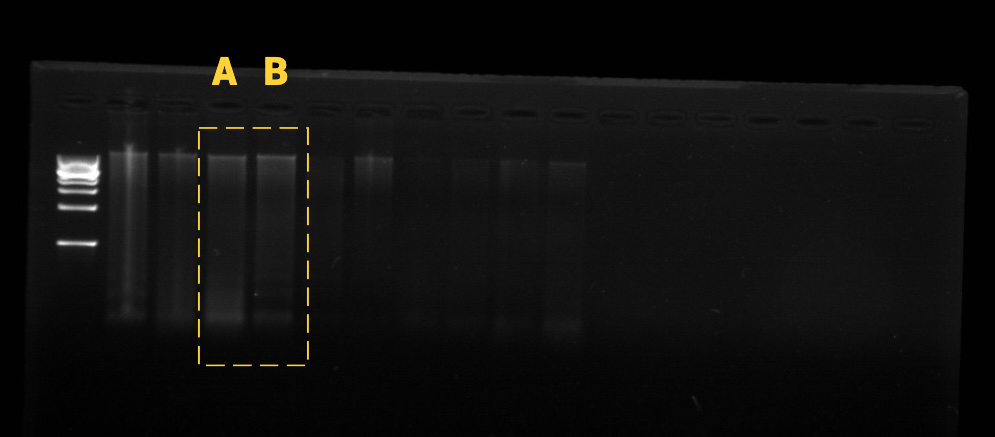
\includegraphics[width=0.8\linewidth]{Figures/20251010_DNA.jpg}
            \caption{Electrophoresis of DNA stock}
        \end{figure}
   \end{block}
    
\end{frame}

\begin{frame}{PCR Primer Design}
    \begin{block}{Universal Primer}
        Universal primer M13 for best sequencing compatibility:
        \begin{itemize}
            \item F:\@5’-TGTAAAACGACGGCCAGT-
            \item R:\@5’-CAGGAAACAGCTATGACC-
        \end{itemize}
    \end{block}
    
    \begin{table}[H]
        \scriptsize
        \centering
        \begin{tabular}{>{\raggedright\arraybackslash}p{0.9cm}>{\raggedright\arraybackslash}p{0.9cm}>{\raggedright\arraybackslash}p{3.8cm}>{\raggedright\arraybackslash}p{0.8cm}>{\raggedright\arraybackslash}p{0.8cm}>{\raggedright\arraybackslash}p{1.1cm}}
            \toprule
            \textbf{Gene} & \textbf{Position} & \textbf{Primer Sequence (5'→3')} & \textbf{T$_m$/\unit{\celsius}} & \textbf{GC\%} & \textbf{Size (bp)} \\
            \midrule
            \makecell[l]{\textit{ALDH2}} & \makecell[l]{1510} & \makecell[l]{F: TGGAGCCCAGTCACCCTTTGGT \\ R: atgggacagagcagaggctggg} & \makecell[l]{61.8 \\ 62.1} & \makecell[l]{59.1 \\ 63.6} & \makecell[l]{413} \\[12pt]
            
            \makecell[l]{\textit{TAS2R38}} & \makecell[l]{145} & \makecell[l]{F: TTTCTGCACTGGGTGGCAACCA \\ R: GCCGGCTGATGCTGAGACACAG} & \makecell[l]{61.2 \\ 62.1 } & \makecell[l]{54.5 \\ 63.6} & \makecell[l]{275} \\[12pt]
            
            \makecell[l]{\textit{TAS2R38}} & \makecell[l]{785/886} & \makecell[l]{F: TGCTCCTGCATCTGCACTGTCC \\ R: CATGCCCAGAGGGACAAGCTGC} & \makecell[l]{61.2 \\ 62.1} & \makecell[l]{59.1 \\ 63.6} & \makecell[l]{433} \\
            \bottomrule
        \end{tabular}
    \end{table}
\end{frame}

\begin{frame}{PCR Amplification}
    \begin{block}{First PCR: Failure}
        \begin{itemize}
            \item No distinct DNA bands in all sample lanes, only faint signals 
            \item Presumably primer degradation
        \end{itemize}
        \begin{figure}
            \centering
            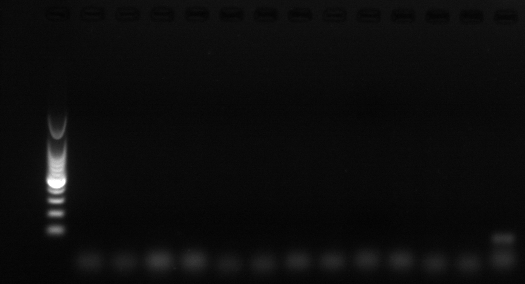
\includegraphics[width=0.8\linewidth]{Figures/20251017_PCR.jpg}
            \caption{Leftmost: marker, rightmost: blank, samples are in between}
        \end{figure}
    \end{block}
\end{frame}

\begin{frame}{PCR Amplification}
    \begin{block}{Second PCR: Success}
        \begin{itemize}
         \item Label: 
      
            Template[\textbf{F}(eng)/\textbf{H}(an)]+Primer[\textbf{A}(LDH2)/\textbf{T}(AS2R38)\textbf{a}/\textbf{T}(AS2R38)\textbf{b}]
            \item Distinct DNA bands in all sample lanes 
            \item Two bands for Tb primer lane: PCR product (top) \& primer dimer (bottom)
            
        \end{itemize}
        \begin{figure}
            \centering
            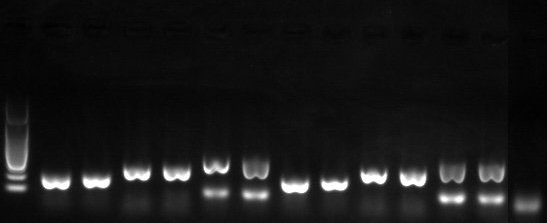
\includegraphics[width=0.8\linewidth]{Figures/20251025_PCR.jpg}
            \caption{L $\to$ R: marker, FA$\times2$, FTa$\times2$, FTb$\times2$, HA$\times2$, HTa$\times2$, HTb$\times2$, blank}
        \end{figure}
    \end{block}
\end{frame}

\begin{frame}{Sequencing Result}
    \setlength{\columnsep}{0.01\textwidth}
    \begin{columns}[T]

    \captionsetup[figure]{font=scriptsize}
        \begin{column}{0.20\textwidth}
            \centering
            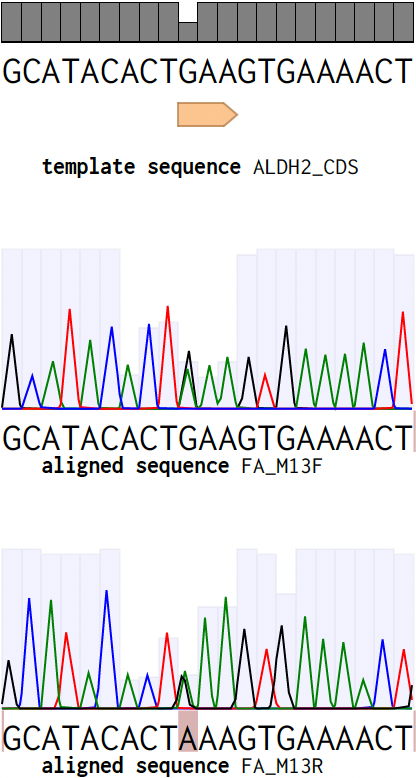
\includegraphics[width=\textwidth]{Figures/FA-1510.png}
            \vspace{-0.5cm}
            \captionof{figure}{FA-1510}
        \end{column}

        \begin{column}{0.20\textwidth}
            \centering
            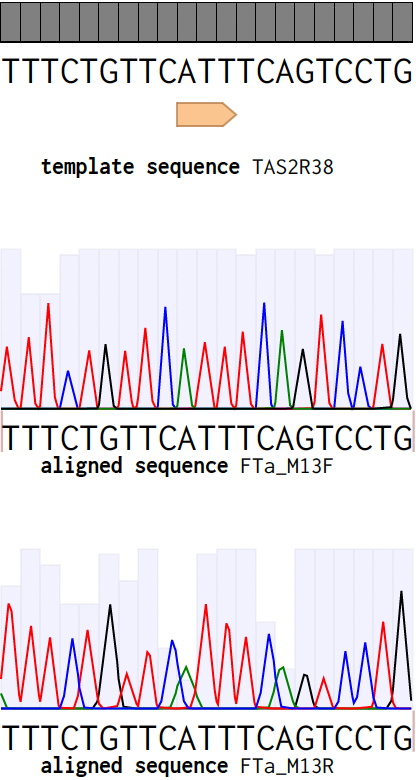
\includegraphics[width=\textwidth]{Figures/FTa-145.png}
            \vspace{-0.5cm}
            \captionof{figure}{FTa-145}
        \end{column}

        \begin{column}{0.20\textwidth}
            \centering
            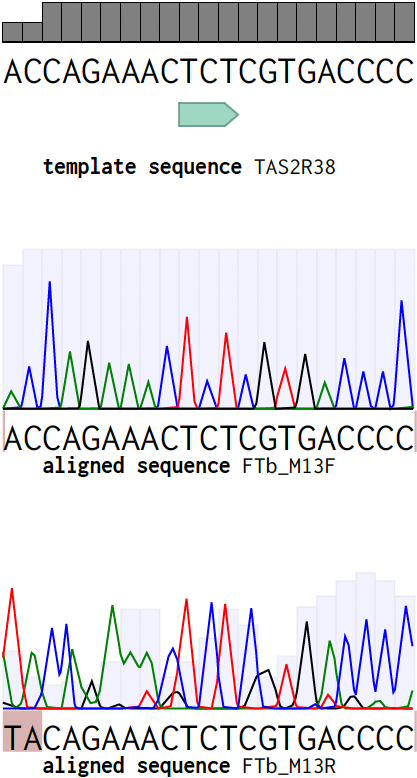
\includegraphics[width=\textwidth]{Figures/FTb-785.png}
            \vspace{-0.5cm}
            \captionof{figure}{FTb-785}
        \end{column}

        \begin{column}{0.20\textwidth}
            \centering
            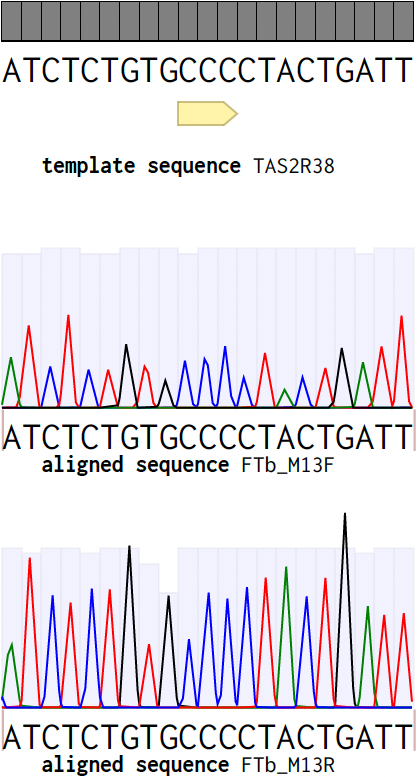
\includegraphics[width=\textwidth]{Figures/FTb-886.png}
            \vspace{-0.5cm}
            \captionof{figure}{FTb-886}
        \end{column}
    \end{columns}

    \vspace{-0.2cm}
    \begin{block}{Sample A (Feng)}
        \begin{itemize}
            \item G/A double peak at \textit{ALDH2} c.1510 $\to$ \textbf{heterozygous G/A (rs671 GA)}
            \item Single A peak at \textit{TAS2R38} c.145 $\to$ \textbf{wild type C/C}
            \item Single C peak at \textit{TAS2R38} c.785 $\to$ \textbf{wild type C/C}
            \item Single C peak at \textit{TAS2R38} c.886 $\to$ \textbf{wild type G/G}
        \end{itemize}
    \end{block}
\end{frame}

\begin{frame}{Sequencing Result}
    \setlength{\columnsep}{0.01\textwidth}
    \begin{columns}[T]

    \captionsetup[figure]{font=scriptsize}
        \begin{column}{0.20\textwidth}
            \centering
            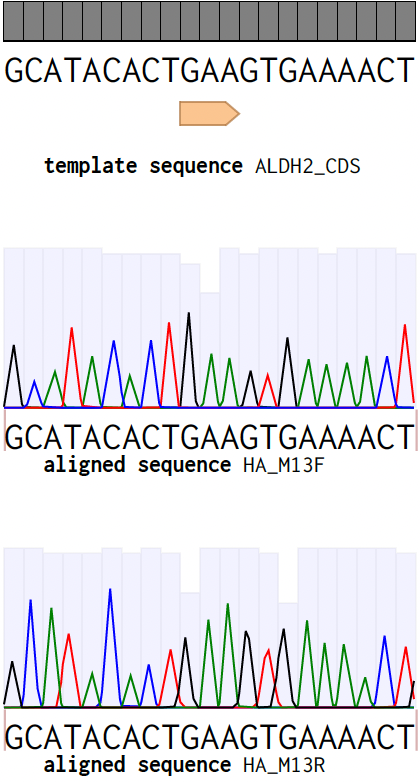
\includegraphics[width=\textwidth]{Figures/HA-1510.png}
            \vspace{-0.5cm}
            \captionof{figure}{FA-1510}
        \end{column}

        \begin{column}{0.20\textwidth}
            \centering
            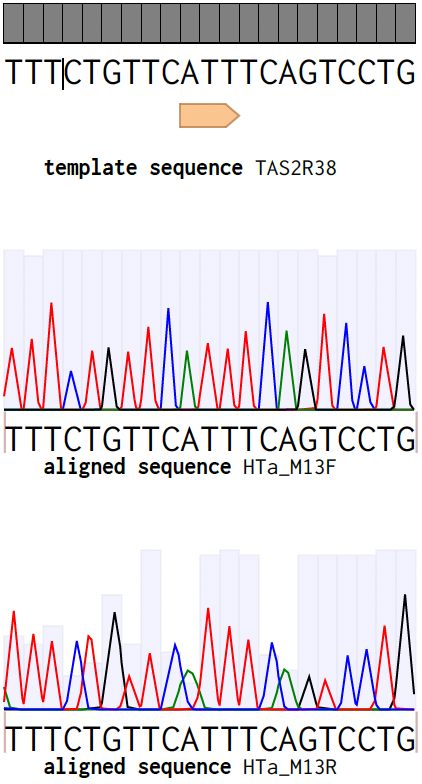
\includegraphics[width=\textwidth]{Figures/HTa-145.png}
            \vspace{-0.5cm}
            \captionof{figure}{FTa-145}
        \end{column}

        \begin{column}{0.20\textwidth}
            \centering
            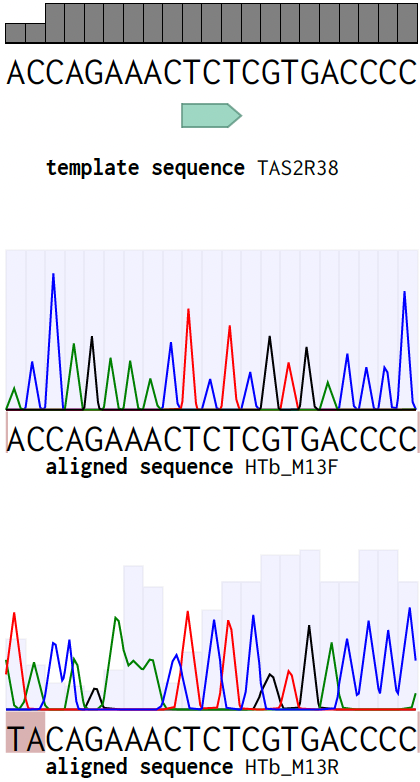
\includegraphics[width=\textwidth]{Figures/HTb-785.png}
            \vspace{-0.5cm}
            \captionof{figure}{FTb-785}
        \end{column}

        \begin{column}{0.20\textwidth}
            \centering
            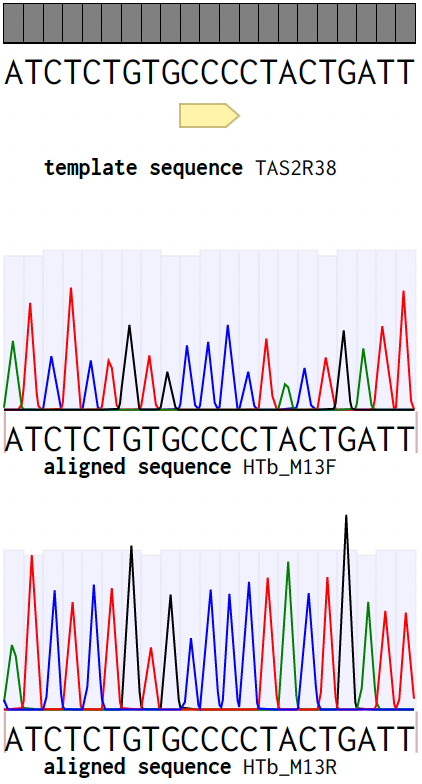
\includegraphics[width=\textwidth]{Figures/HTb-886.png}
            \vspace{-0.5cm}
            \captionof{figure}{FTb-886}
        \end{column}
    \end{columns}

    \vspace{-0.2cm}
    \begin{block}{Sample B (Han)}
        \begin{itemize}
            \item Single G peak at \textit{ALDH2} c.1510 $\to$ \textbf{wild type G/G}
            \item Single A peak at \textit{TAS2R38} c.145 $\to$ \textbf{wild type C/C}
            \item Single C peak at \textit{TAS2R38} c.785 $\to$ \textbf{wild type C/C}
            \item Single C peak at \textit{TAS2R38} c.886 $\to$ \textbf{wild type G/G}
        \end{itemize}
    \end{block}
\end{frame}

\begin{frame}{Phylogenetic Trees}
    \begin{block}{Sources \& Presets}
        \begin{itemize}
            \item 22 species: Human, Chimp, Gorilla, Gibbon, Green Monkey, Rhesus, Marmoset, Mouse Lemur, Mouse, Rat, Rabbit, Hedgehog, Pig, Cow, Sheep, Dolphin, Horse, Dog, Panda, Cat, Elephant, Armadillo
            \item 3 methods: Neighbor Joining (NJ), Maximum Parsimony (MP), Maximum Likelihood (ML)
            \item 1000 times bootstrap tests
            \item Generate using MEGA 12
        \end{itemize}
    \end{block} 
\end{frame}

\begin{frame}{Phylogenetic Trees}
    \begin{minipage}[h]{0.49\textwidth}
        \centering
        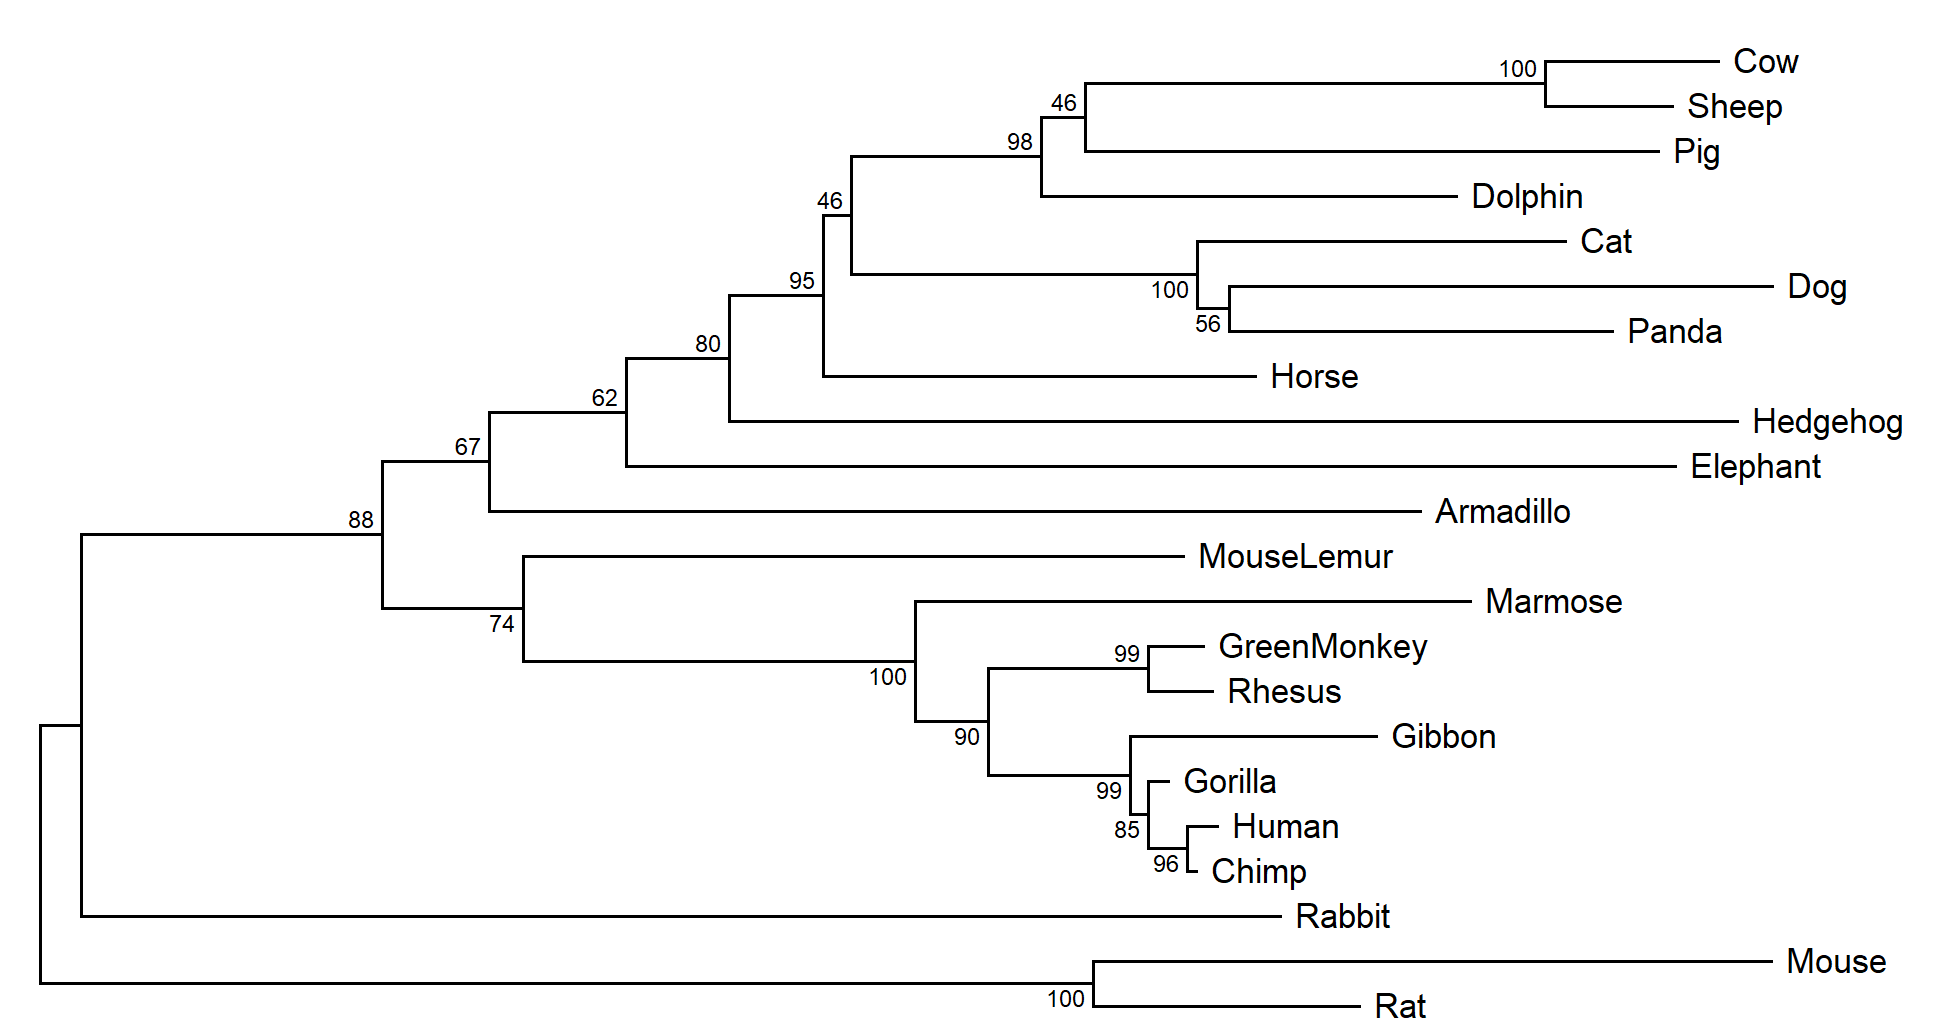
\includegraphics[width=\linewidth]{Figures/ALDH2_ML.png}
    \end{minipage}
    \hfill
    \begin{minipage}[h]{0.49\textwidth}
        \centering
        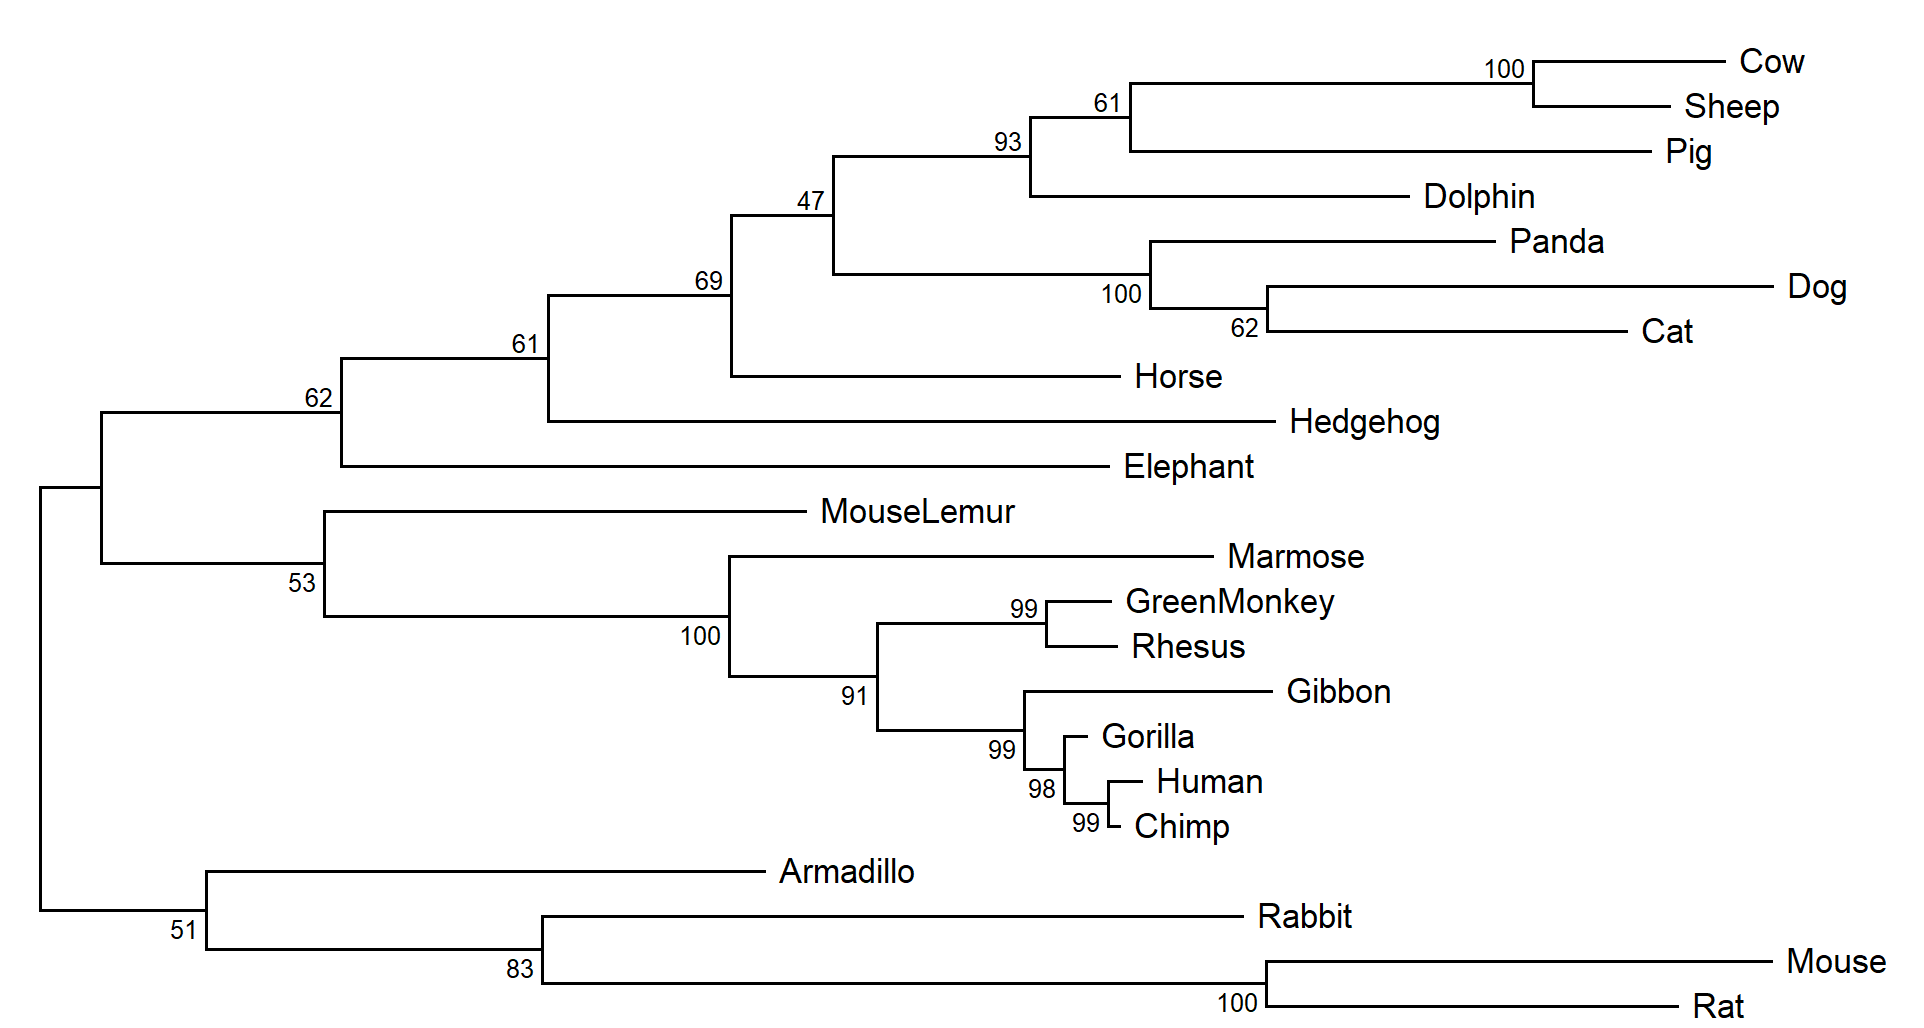
\includegraphics[width=\linewidth]{Figures/ALDH2_MP.png}
    \end{minipage}
    
    \vspace{0.5cm}

    \begin{minipage}[h]{0.49\textwidth}
        \centering
        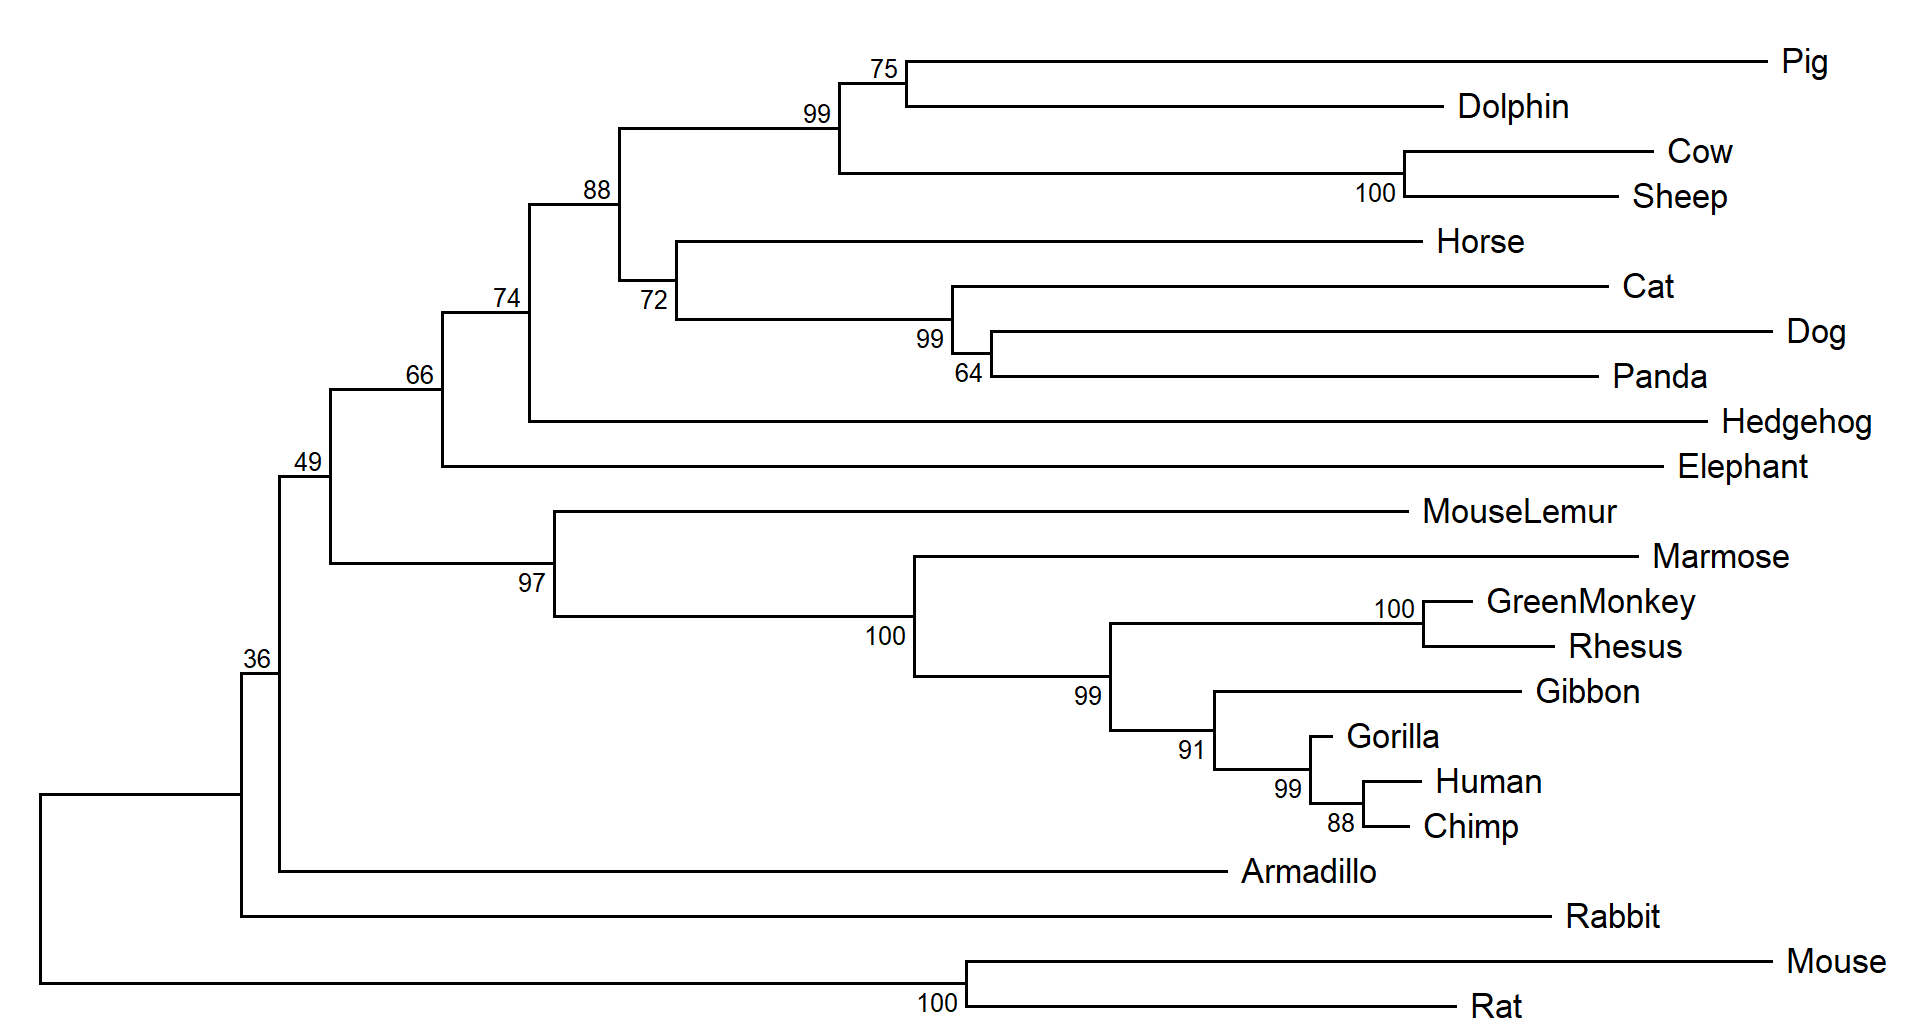
\includegraphics[width=\linewidth]{Figures/ALDH2_NJ.png}
    \end{minipage}
    \hspace{0.7cm}
    \begin{minipage}[h]{0.4\textwidth}
        \raggedright
        \textbf{Phylogeny of \textit{ALDH2}}
        \begin{itemize}
            \item Top-left: ML method
            \item Top-right: MP method
            \item Bottom-left: NJ method
        \end{itemize}
    \end{minipage}
\end{frame}

\begin{frame}{Phylogenetic Trees}
    \begin{minipage}[h]{0.49\textwidth}
        \centering
        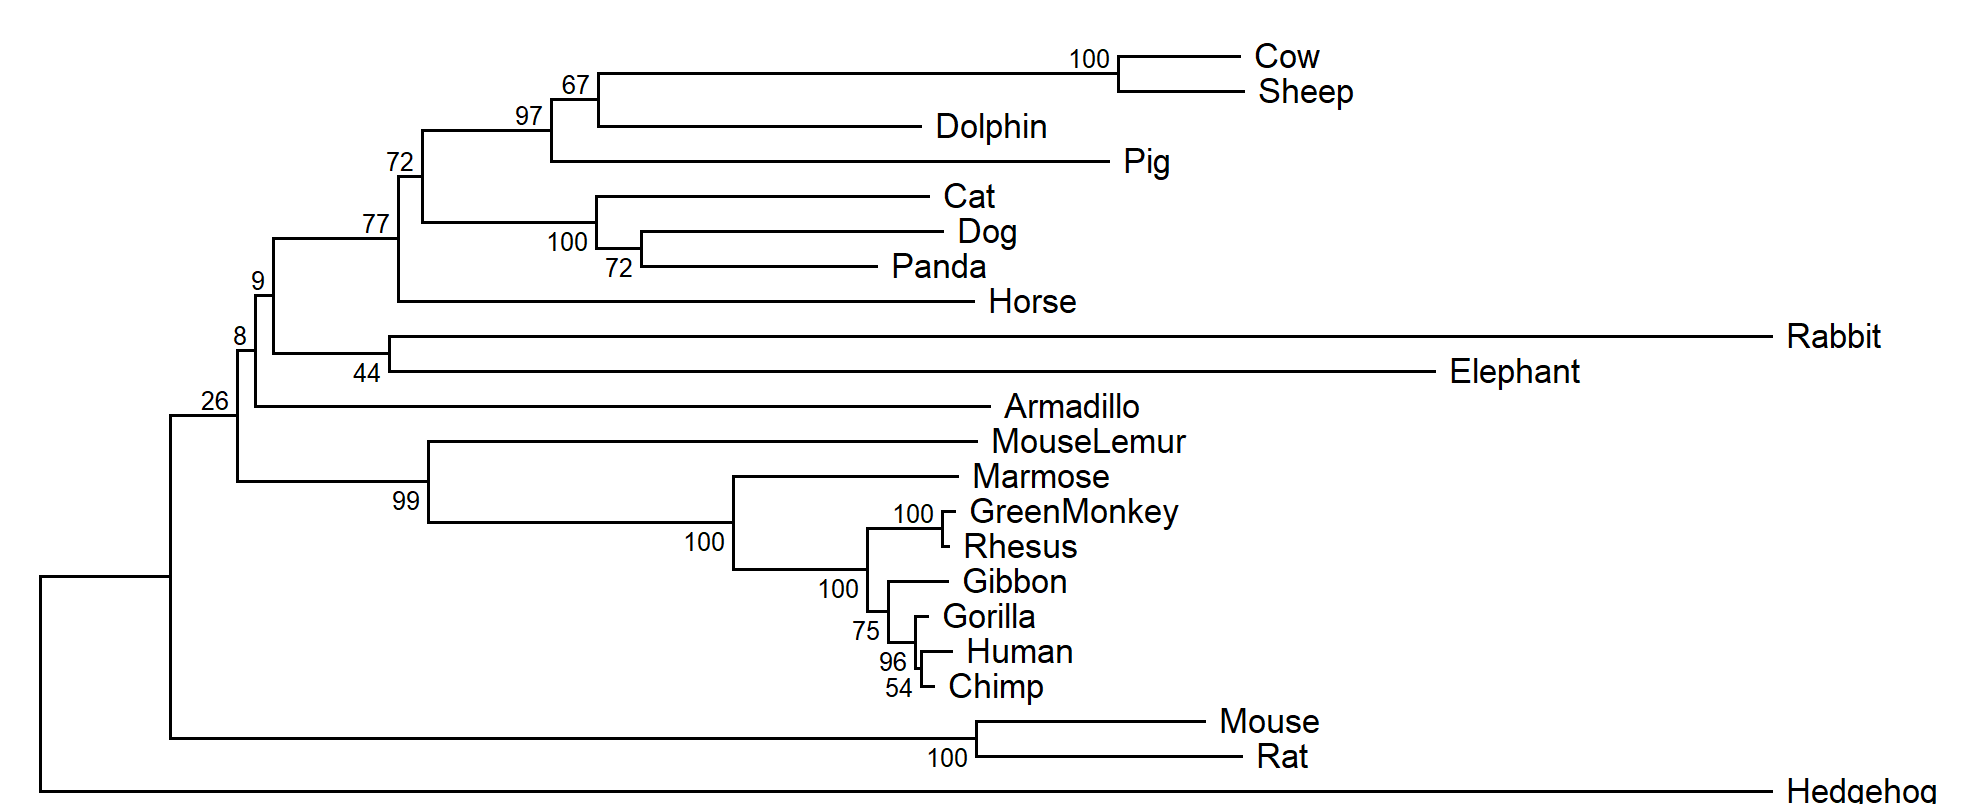
\includegraphics[width=\linewidth]{Figures/TAS2R38_ML.png}
    \end{minipage}
    \hfill
    \begin{minipage}[h]{0.49\textwidth}
        \centering
        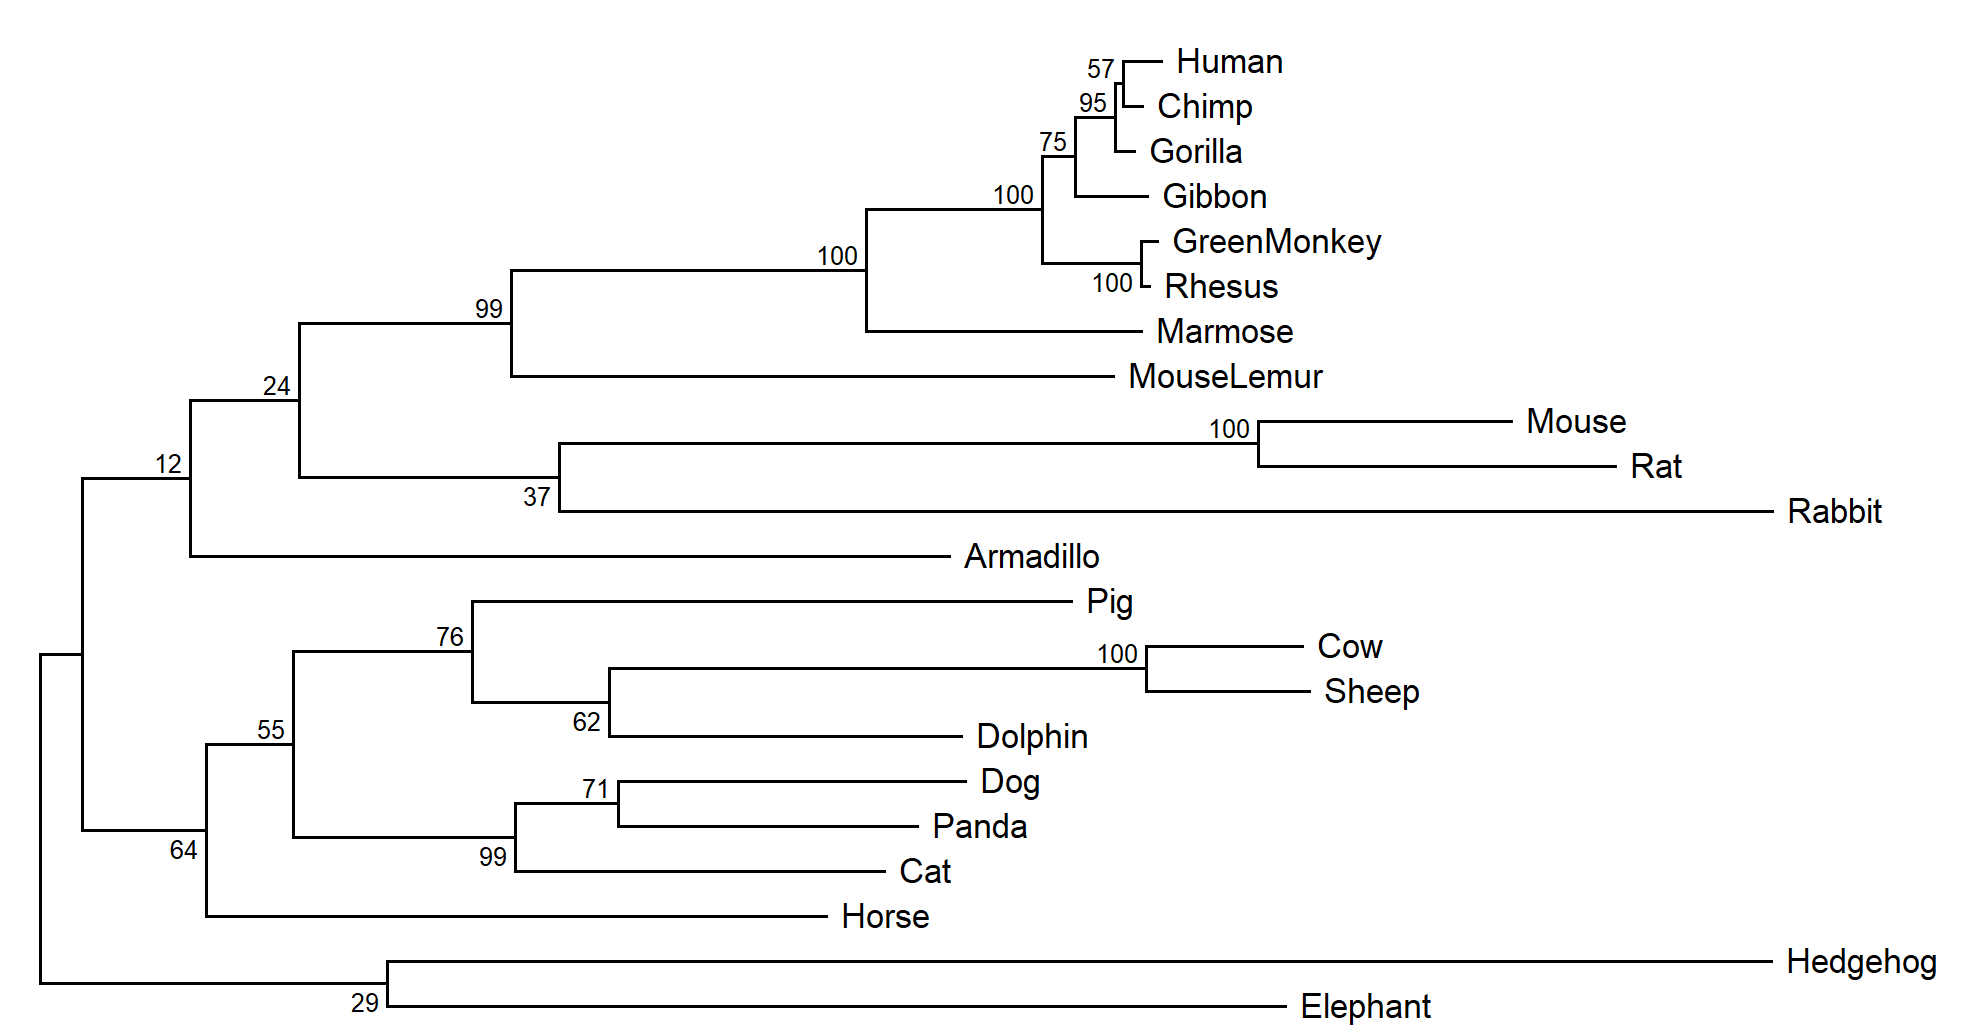
\includegraphics[width=\linewidth]{Figures/TAS2R38_MP.png}
    \end{minipage}
    
    \vspace{0.5cm}

    \begin{minipage}[h]{0.49\textwidth}
        \centering
        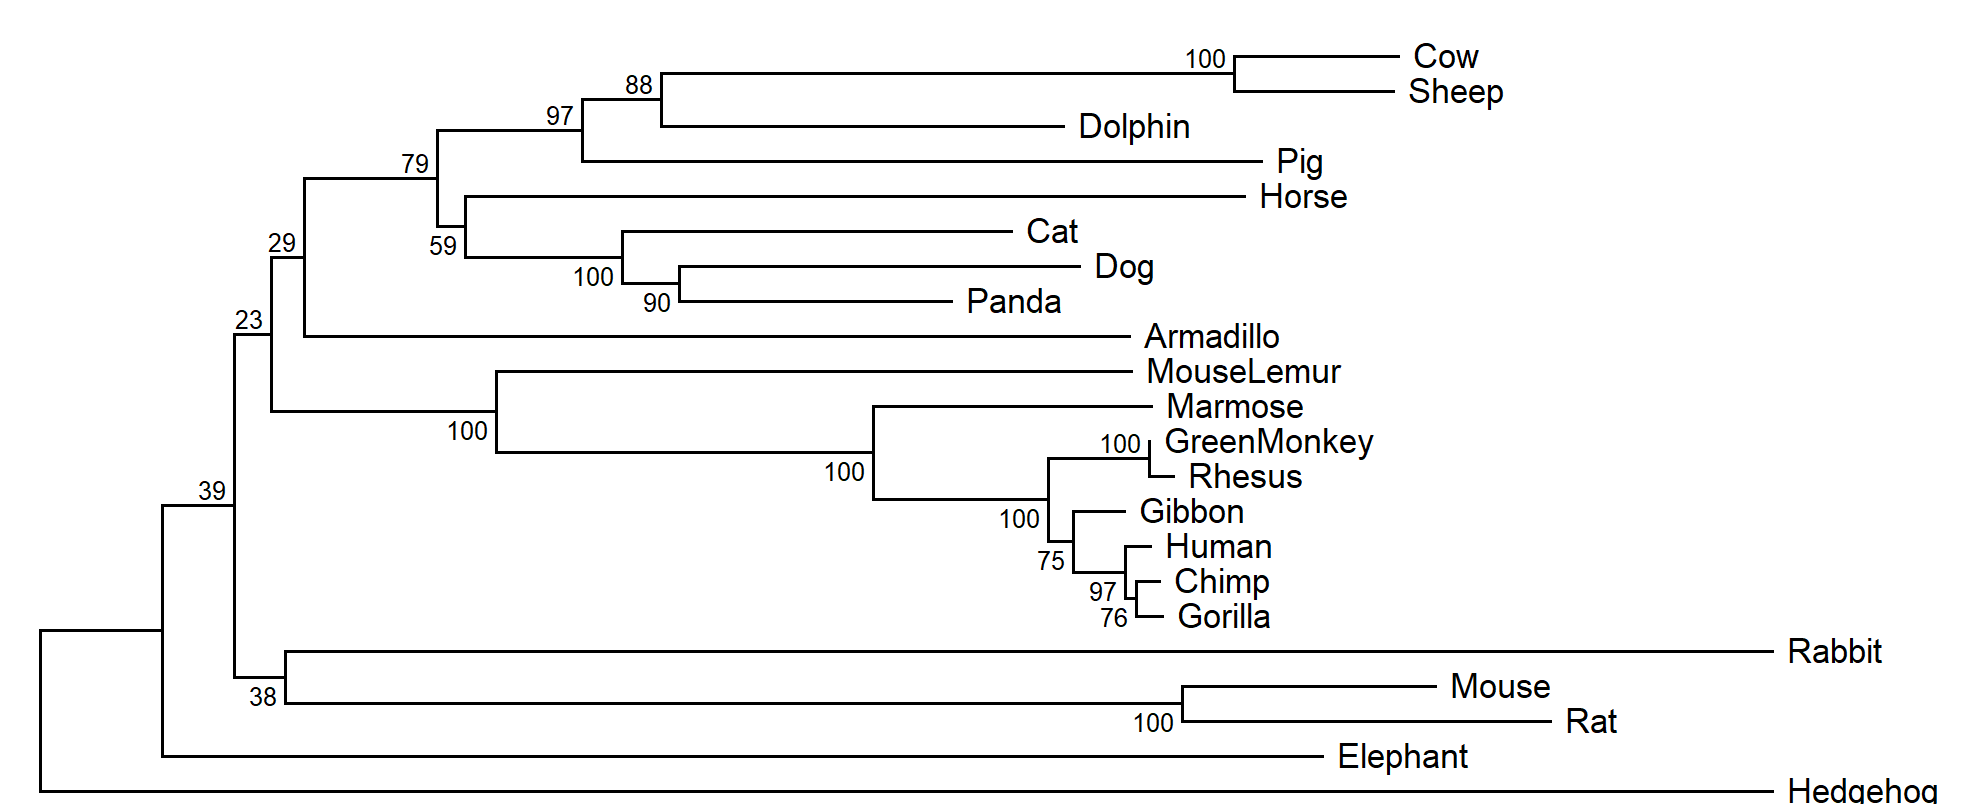
\includegraphics[width=\linewidth]{Figures/TAS2R38_NJ.png}
    \end{minipage}
    \hspace{0.7cm}
    \begin{minipage}[h]{0.4\textwidth}
        \raggedright
        \textbf{Phylogeny of \textit{TAS2R38}}
        \begin{itemize}
            \item Top-left: ML method
            \item Top-right: MP method
            \item Bottom-left: NJ method
        \end{itemize}
    \end{minipage}
\end{frame}

\section{Discussion}

% \begin{frame}{Phenotype-Genotype Correlation}    
%     \begin{table}[H]
%     \scriptsize
%     \centering
%         \begin{tabular}{>{\raggedright\arraybackslash}p{0.7cm}>{\raggedright\arraybackslash}p{1.7cm}>{\raggedright\arraybackslash}p{1.6cm}>{\raggedright\arraybackslash}p{2.4cm}>{\raggedright\arraybackslash}p{2cm}}
%             \toprule
%             \textbf{Sample} & \textbf{Site} & \textbf{Genotype} & \textbf{Predicted Phenotype} & \textbf{Actual Phenotype}\\
%             \midrule
            
%             \multirow{4}{*}{\makecell[l]{Zhang}} 
%             & \textit{ALDH2} c.1510 & Wild Type G/G & Normal aldehyde metabolism & Do not flush when drinking \\
%             \cmidrule(lr){2-5} % 添加横线，从第2列到第5列
%             & \textit{TAS2R38} c.145 & Wild Type A/A & &  \\
%             & \textit{TAS2R38} c.785 & Wild Type C/C & Strong bitter taste & Slightly bitter \\
%             & \textit{TAS2R38} c.886 & Wild Type C/C & &  \\
            
%             \midrule

%             \multirow{4}{*}{\makecell[l]{Liu}} 
%             & \textit{ALDH2} c.1510 & Wild Type G/G & Normal aldehyde metabolism & Do not flush when drinking \\
%             \cmidrule(lr){2-5} % 添加横线，从第2列到第5列
%             & \textit{TAS2R38} c.145 & Wild Type A/A & &  \\
%             & \textit{TAS2R38} c.785 & Wild Type C/C & Strong bitter taste & Slightly bitter \\
%             & \textit{TAS2R38} c.886 & Wild Type C/C & &  \\

%             \midrule
       
%             \multirow{4}{*}{\makecell[l]{Jiang}} 
%             & \textit{ALDH2} c.1510 & Heterozygous G/A & Aldehyde metabolism disorder & No alcohol consumption \\
%             \cmidrule(lr){2-5} % 添加横线，从第2列到第5列
%             & \textit{TAS2R38} c.145 & Wild Type A/A & &  \\
%             & \textit{TAS2R38} c.785 & Wild Type C/C & Strong bitter taste & Slightly bitter \\
%             & \textit{TAS2R38} c.886 & Wild Type C/C & &  \\
%             \bottomrule
%         \end{tabular}
%     \end{table}
%\end{frame}

\begin{frame}{Phenotype-Genotype Correlation}    
    \begin{table}[H]
    \scriptsize
    \centering
        \begin{tabular}{>{\raggedright\arraybackslash}p{0.7cm}>{\raggedright\arraybackslash}p{1.7cm}>{\raggedright\arraybackslash}p{1.6cm}>{\raggedright\arraybackslash}p{2.4cm}>{\raggedright\arraybackslash}p{2cm}}
            \toprule
            \textbf{Sample} & \textbf{Site} & \textbf{Genotype} & \textbf{Predicted Phenotype} & \textbf{Actual Phenotype}\\
            \midrule
            
            \multirow{4}{*}{\makecell[l]{Han}} 
            & \textit{ALDH2} c.1510 & Wild Type G/G & Normal aldehyde metabolism & No alcohol consumption \\
            \cmidrule(lr){2-5} % 添加横线，从第2列到第5列
            & \textit{TAS2R38} c.145 & Wild Type C/C & &  \\
            & \textit{TAS2R38} c.785 & Wild Type C/C & Strong bitter taste & Slightly bitter \\
            & \textit{TAS2R38} c.886 & Wild Type G/G & &  \\
            
            \midrule

            \multirow{4}{*}{\makecell[l]{Feng}} 
            & \textit{ALDH2} c.1510 & Heterozygous G/A & Aldehyde metabolism disorder & Flush when drinking \\
            \cmidrule(lr){2-5} % 添加横线，从第2列到第5列
            & \textit{TAS2R38} c.145 & Wild Type C/C & &  \\
            & \textit{TAS2R38} c.785 & Wild Type C/C & Strong bitter taste & Slightly bitter \\
            & \textit{TAS2R38} c.886 & Wild Type G/G & &  \\
            \bottomrule
        \end{tabular}
    \end{table}
    \vspace{0.5cm}
    \begin{itemize}
        \item Good correlation between genotypes and phenotypes for \textit{ALDH2}
        \item Contradiction between genotypes and phenotypes for \textit{TAS2R38}
    \end{itemize}
\end{frame}

\begin{frame}{\textit{ALDH2$^*$ 504Lys}}
    \begin{block}{Overview}
        \begin{itemize}
            \item Mitochondrial aldehyde dehydrogenase (\textit{ALDH2}) is one of the most important enzymes in human alcohol metabolism. 
            \item The \textit{ALDH2$^*$2 504Lys} variant (\textit{rs671}) takes place at c.1510 (G $\to$ A) and substitutes \textbf{Glu} to \textbf{Lys} at residue 504.
            \item Inherited as an autosomal dominant trait:
            \begin{itemize}
                \item Glu504 homozygotes (ALDH2*1/1) exhibit normal enzymatic activity
                \item Glu504/Lys504 heterozygotes (ALDH2*1/2) show approximately 6\% of normal activity \citep{xiaoMutationMitochondrialAldehyde1996}
                \item Lys504 homozygotes (ALDH2*2/2) show negligible activity toward acetaldehyde \citep{crabbGenotypesAldehydeDehydrogenase1989}
            \end{itemize}
        \end{itemize}
    \end{block}
\end{frame}

\begin{frame}{\textit{ALDH2$^*$ 504Lys}}
    \begin{block}{Molecular Mechanism}
        \vspace{0.4cm}
        \hfill
        \begin{minipage}[h]{0.35\textwidth}
            \centering
            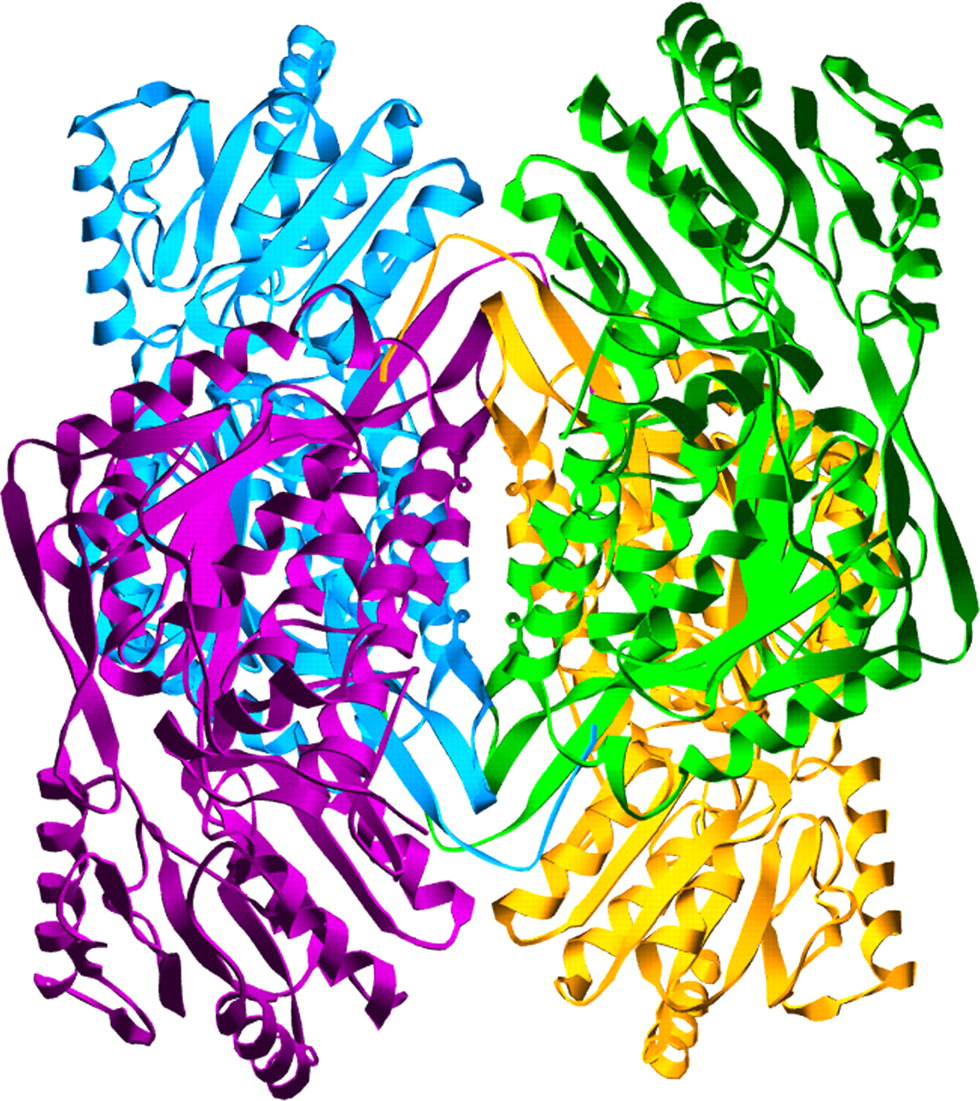
\includegraphics[width=0.9\linewidth]{Figures/gr1_lrg.jpg}
            \captionof{figure}{\textit{ALDH2} tetramer}
        \end{minipage}
        \begin{minipage}[h]{0.60\textwidth}
            Glu504 (negatively charged) to Lys (positively charged) substitution disrupts a critical salt bridge and hydrogen-bonding network at the tetramerization interface. This not only destabilizes the tetramer but also distorts the geometry of the catalytic and coenzyme(NAD$^+$)-binding sites in adjacent subunits. \citep{larsonDisruptionCoenzymeBinding2005}
        \end{minipage}

        \hspace{0.1cm}
        \begin{minipage}[h]{0.96\textwidth}
            \citet{larsonDisruptionCoenzymeBinding2005} state that the mutation ``results in a complete loss of activity'', and the dominant-negative effect occurs because ``the incorporation of even a single subunit... is sufficient to destabilize the tetramer and inactivate the enzyme''.
        \end{minipage}
    \end{block}
\end{frame}

\begin{frame}{\textit{ALDH2$^*$ 504Lys}}
    Only one sample (Feng, fr. Zhejiang) among five harbored a mutation at \textit{ALDH2} c.1510, characterized as a \textbf{G/A heterozygote}.

    \begin{minipage}[h]{0.54\textwidth}
        \centering
        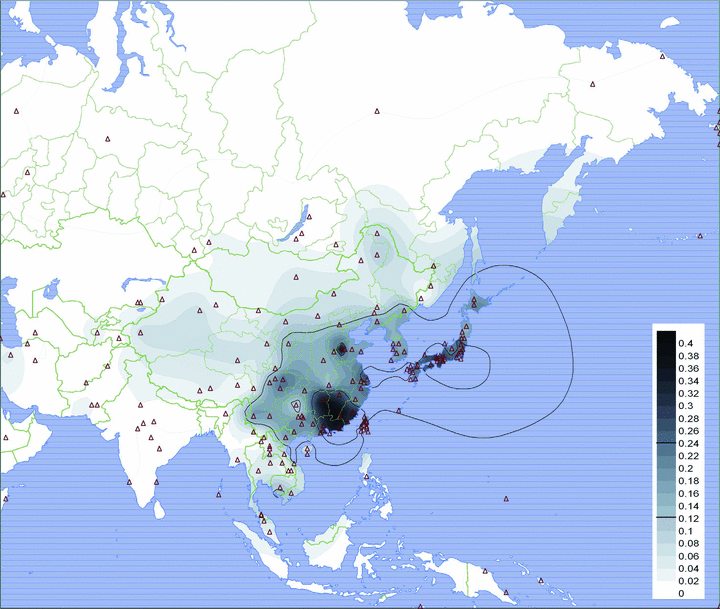
\includegraphics[width=0.9\linewidth]{Figures/ALDH2 504Lys Distribution.png}
        \captionof{figure}{\textit{ALDH2$^*$ 504Lys} distribution}
    \end{minipage}
    \hfill
    \begin{minipage}[h]{0.43\textwidth}
        \vspace{-0.5cm}
        \begin{block}{Geo-Distribution}
             \citet{liRefinedGeographicDistribution2009a} reported the variant to be \textbf{essentially exclusive to East Asia}, and the highest frequency (up to 40.9\%) was found in \textbf{Southeastern China}.

            The expansion and genetic influence of the Han Chinese spread the allele throughout East Asia.
        \end{block}
    \end{minipage}
\end{frame}

\begin{frame}{\textit{ALDH2$^*$ 504Lys}}
    \begin{block}{Evolution History}
        \citet{liRefinedGeographicDistribution2009a} concluded that allele was likely originated in ancient Han Chinese in Central China, although being found most abundant in Southeastern China.
        \begin{itemize}
            \item Indigenous populations in South China (e.g., Hmong-Mien, Daic groups like Kam and Laka) and the aboriginal peoples of Taiwan and Hainan have \textbf{very low or absent} frequencies of the allele.
            \item Historical and genetic data show these groups are descendants of migrants from Central China. The high frequency was \textbf{carried} and \textbf{maintained} by these migrants, not originated in the south.
            \item Historically, Altaic populations (e.g., Xianbei, Huns, Khitans, Jurchens) moved into Central China. Since modern Altaic populations have very low \textit{ALDH2$^*$ 504Lys} frequencies, their integration into the Central Chinese gene pool would have diluted the allele's frequency in its place of origin.
        \end{itemize} 
    \end{block}
\end{frame}

\begin{frame}{\textit{ALDH2$^*$ 504Lys}}
    \begin{block}{Evolution History}
        \begin{itemize}   
            \item The Han Chinese migrants who moved south may have experienced:
            \begin{itemize}
                \item Founder effect: The migrating groups carried a high frequency of the allele.
                \item Protection against severe alcoholism: In ancient agrarian societies, even a modest reduction in alcohol consumption could have conferred significant survival and reproductive advantages by preventing liver disease, accidents, and social strife.
            \end{itemize}
        \end{itemize} 
    \end{block}
        
    \begin{block}{Associatied Diseases}
        \begin{itemize}
            \item Cardiovascular Disease: \textit{ALDH2} is the primary enzyme responsible for converting nitroglycerin to nitric oxide. \textit{ALDH2$^*$ 504Lys} carriers show a significantly blunted response to nitroglycerin, a major issue in cardiovascular pharmacogenetics. \citep{liMitochondrialAldehydeDehydrogenase22006}
            \item Cancer Relations: Cancer incidences increase among alcoholics in organs including esophagus, stomach, liver, upper aerodigestive tract in which acetaldehyde is produced by the alcohol dehydrogenases. \citep{yokoyamaAlcoholAldehydeDehydrogenase2001}
        \end{itemize}
    \end{block}
\end{frame}

\begin{frame}{\textit{TAS2R38} SNPs}
    \begin{block}{Overview}
        \begin{itemize}
            \item TAS2R38 encodes a G protein-coupled bitter taste receptor protein found on the plasma membrane of taste cells, which determines an individual's ability to taste certain bitter compounds like 6-n-propylthiouracil (PROP) and phenylthiocarbamide (PTC).
            \item Contain 3 common SNPs:
            \begin{itemize}
                \item \textit{rs713598}: Pro $\to$ Ala at 49; 
                \item \textit{rs1726866}: Ala $\to$ Val at 262; 
                \item \textit{rs10246939}: Val $\to$ Ile at 296.
            \end{itemize}
            \item Strong linkage disequilibrium \citep{rissoGlobalDiversityTAS2R382016}, forming 2 common observable haplotypes: PAV (the “taster” allele) and AVI (the “non-taster” allele).
        \end{itemize}
    \end{block}
\end{frame}

\begin{frame}{\textit{TAS2R38} SNPs}
    \begin{block}{Molecular Mechanism}
        \begin{itemize}
            \item \textit{TAS2R38} encodes a Class A GPCR expressed in type II taste receptor cells of the tongue.
            \item \textit{TAS2R38} responds to compounds containing \textbf{N-C=S moiety}. \citep{bufeMolecularBasisIndividual2005}
            
            \begin{center}
                
\includegraphics[width=0.5\linewidth]{Figures/PTCPROP.png}
            \end{center}
            
            \item Signaling cascade: \citep{chandrashekarT2RsFunctionBitter2000,zhangCodingSweetBitter2003}
            
            Ligands bind \textit{TAS2R38} $\to$ Receptor conformational change $\to$ 
            G protein (Gustducin) activation $\to$ PLC$\beta$2 $\to$ IP$_3$ $\to$ 
            Ca$^{2+}$ release $\to$ TRPM5 activation $\to$ Depolarization $\to$ Neural signal

        \end{itemize}
    \end{block}
\end{frame}

\begin{frame}{\textit{TAS2R38} SNPs}
    \begin{block}{Molecular Mechanism}
        \begin{itemize}
            \item \citet{bufeMolecularBasisIndividual2005} stated that \textbf{P49A and A262V} affect cellular respoding most:
            \begin{itemize}
                \item AVI\&AVV variants do not respond to PTC/PROP;
                \item PAV\&PAI variants respond equally storng.
            \end{itemize}
            \item The AVI receptor has a distorted or less accessible binding pocket, leading to poor ligand binding and weak conformational activation. \citep{biarnesInsightsBindingPhenyltiocarbamide2010}

            \begin{center}
                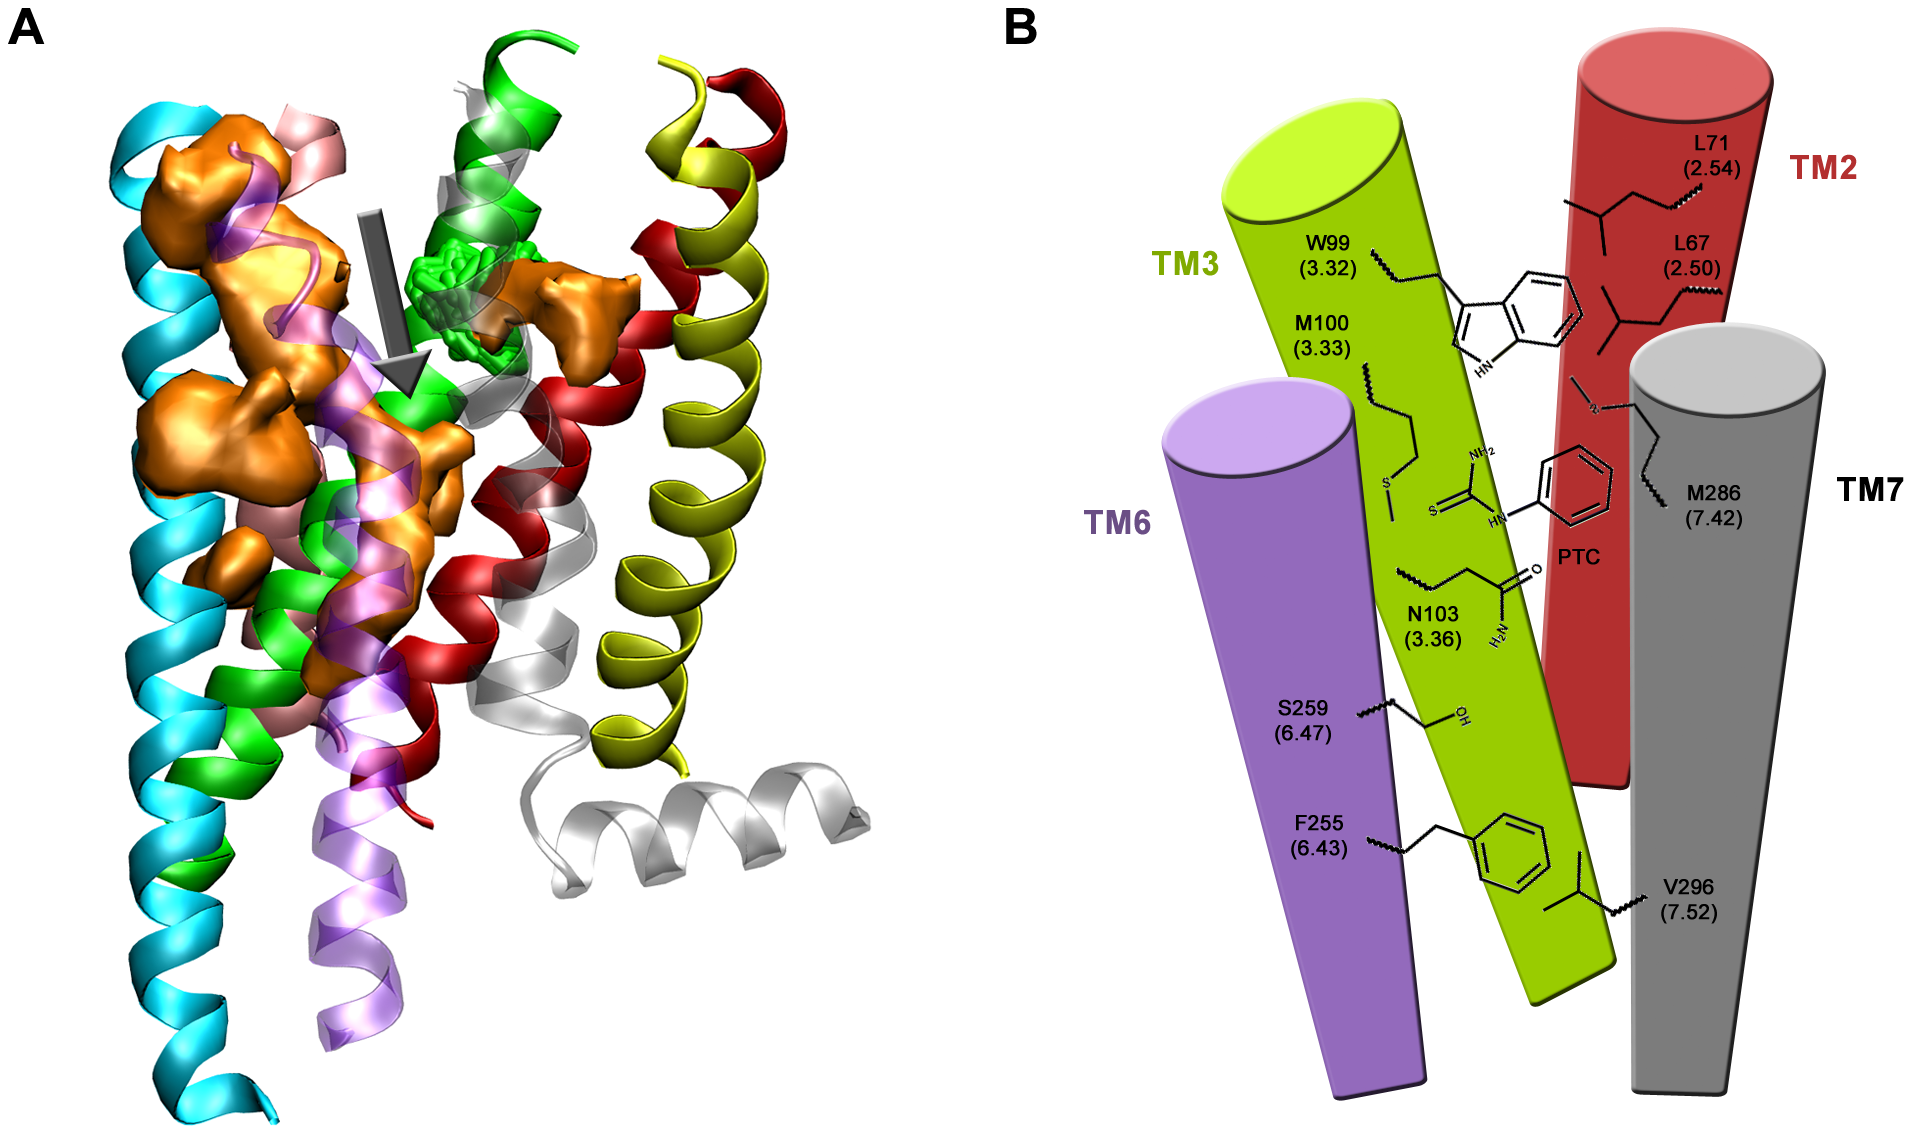
\includegraphics[width=0.6\textwidth]{Figures/TAS2R38.png}
            \end{center}

        \end{itemize}
    \end{block}
\end{frame}

\begin{frame}{\textit{TAS2R38} SNPs}
    \begin{block}{Distribution \& Evolution}
        \begin{center}
            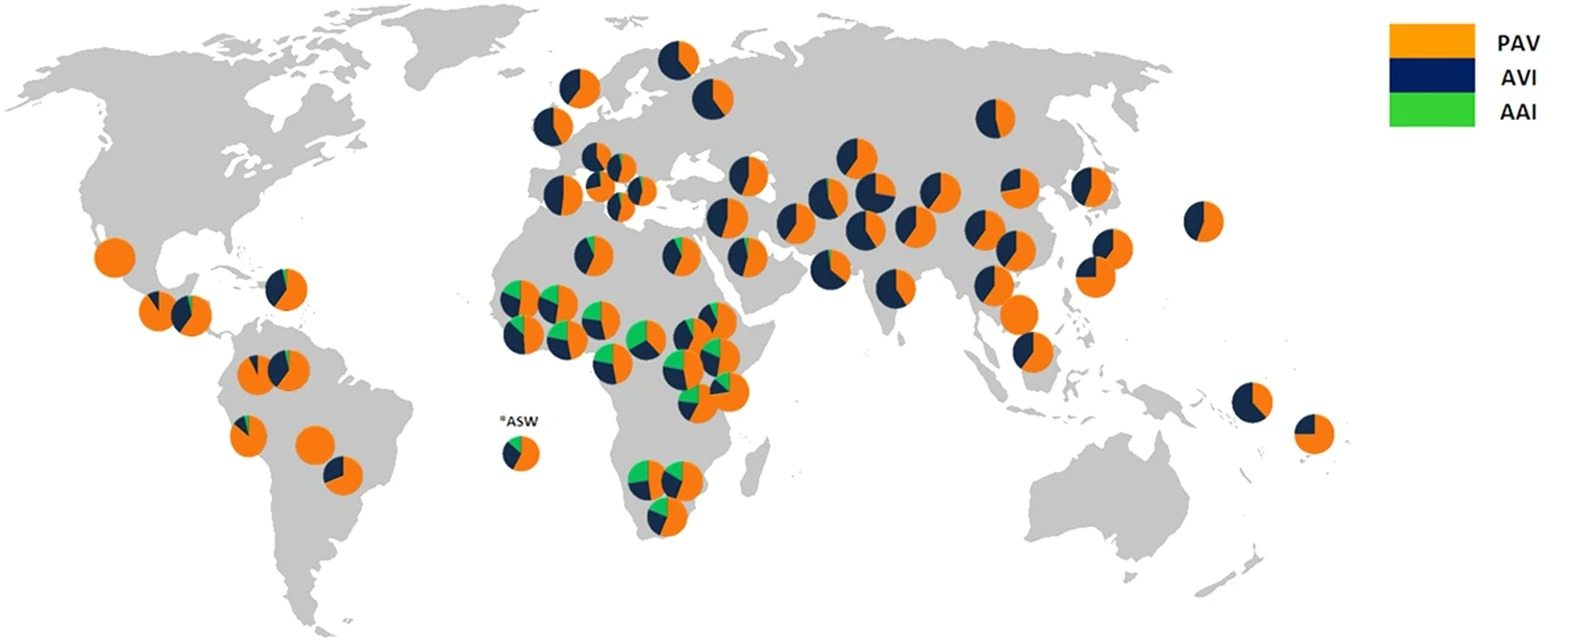
\includegraphics[width=0.6\textwidth]{Figures/TAS2R38_Dis.jpg}
            \captionof{figure}{TAS2R38 variant distribution \citep{rissoGlobalDiversityTAS2R382016}}
        \end{center}

        \begin{itemize}
            \item All 5 samples exhibit wild type, which supports the statistics that PAV variant (wild type) is more prevalent in Asian area. 
            \item \citet{rissoGlobalDiversityTAS2R382016} propose “ancient balancing selection acting...before the Out-Of-Africa event, that maintained both PAV and AVI alleles at roughly the same frequency” because they may be “important for detecting potentially toxic bitter compounds found uniquely in the African continent”.
        \end{itemize}
    \end{block}
\end{frame}
\begin{frame}[allowframebreaks]{References}
    \renewcommand*{\bibfont}{\footnotesize}
    \bibliography{ref}
    \bibliographystyle{apalike}
    % \tiny\bibliographystyle{alpha}
\end{frame}

\begin{frame}
    \begin{center}
        {\Huge\calligra Thanks!}
    \end{center}
\end{frame}

\end{document}